% Created 2025-06-23 Mon 07:47
% Intended LaTeX compiler: pdflatex
\documentclass[bigger]{beamer}
\usepackage[utf8]{inputenc}
\usepackage[T1]{fontenc}
\usepackage{graphicx}
\usepackage{longtable}
\usepackage{wrapfig}
\usepackage{rotating}
\usepackage[normalem]{ulem}
\usepackage{amsmath}
\usepackage{amssymb}
\usepackage{capt-of}
\usepackage{hyperref}
\usetheme[height=20pt]{Arguelles}
\author{Wallysson Oliveira, Leonardo Valente, Lucas Bortoleto}
\date{}
\title{GNU Guix}
\subtitle{Gerenciador de pacotes transacional e Distribuição}
\hypersetup{
 pdfauthor={Wallysson Oliveira, Leonardo Valente, Lucas Bortoleto},
 pdftitle={GNU Guix},
 pdfkeywords={},
 pdfsubject={},
 pdfcreator={Emacs 30.1 (Org mode 9.7.25)}, 
 pdflang={Pt-Br}}
\begin{document}

\maketitle
\begin{frame}[label={sec:org1ab6533}]{O que é o projeto GNU?}
\href{https://www.gnu.org/home.en.html}{GNU} é um sistema operacional livre, ou seja, que respeita a liberdade de seus usuários.

O sistema operacional GNU consiste em pacotes GNU (programas especificamente lançados pelo Projeto GNU)
bem como software livre lançado por terceiros.

O desenvolvimento do GNU tornou possível o uso de um computador sem um software que ameace sua liberdade.

O gerenciador de pacotes e distribuição (GNU/Linux, Hurd) \href{https://guix.gnu.org/}{Guix} faz parte do projeto GNU.
\end{frame}
\begin{frame}[label={sec:org3b6ca69},fragile]{O que é um gerenciador de pacotes transacional?}
 Tal como um Banco de Dados, cada operação de um gerenciador de pacotes transacional é uma transação, ou seja,
ou a operação é um sucesso ou nada acontece (o estado atual é mantido).

\href{https://guix.gnu.org/manual/en/html\_node/Package-Management.html}{Guix} também mantém cada estado salvo, chamados de gerações, permitindo ao usuário "voltar no tempo" com
o comando:
\begin{verbatim}
guix package -S [PATTERN]
\end{verbatim}
Onde PATTERN é um REGEX.

Você pode listar as gerações com o comando:
\begin{verbatim}
guix package -l [PATTERN]
\end{verbatim}
Caso nenhum PATTERN seja enviado, Guix irá mostrar todas as gerações.
\end{frame}
\begin{frame}[label={sec:orge490e68}]{Exemplo:}
\begin{minipage}[c]{0.45\textwidth}
  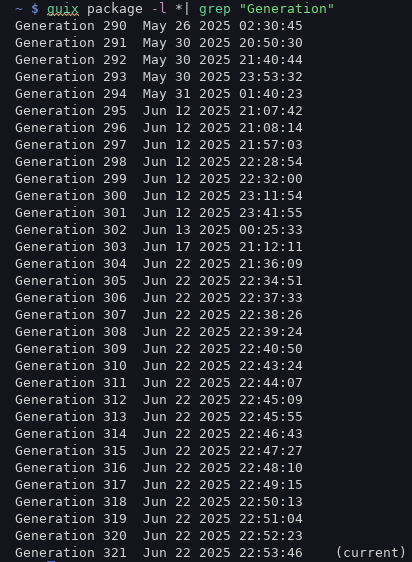
\includegraphics[height=1.5\textwidth]{~/Unicamp/MC504/Apresentação Guix/List generations.png}
\end{minipage}%
\hfill
\begin{minipage}[c]{0.45\textwidth}
  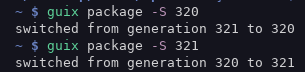
\includegraphics[height=0.25\textwidth]{~/Unicamp/MC504/Apresentação Guix/Switch generation.png}
\end{minipage}
\end{frame}
\begin{frame}[label={sec:orgdd0cd8a},fragile]{Mas isso não ocupa muito armazenamento?}
 A resposta curta é: Sim!

A resposta longa é: Sim! E por isso Guix vem equipado com um Coletor de Lixo que pode ser executado pelo
usuário a qualquer comando através do comando:
\begin{verbatim}
guix gc
\end{verbatim}

Guix consegue determinar quais pacotes ainda são utilizados através dos perfis e remover aqueles que
não estão mais em uso.

Além disso, o coletor de lixo pode também remover gerações muito antigas, as quais o usuário possivelmente não
irá querer voltar, através do comando:
\begin{verbatim}
guix gc -d [PATTERN]
\end{verbatim}
\end{frame}
\begin{frame}[label={sec:orgeb2b8c7},fragile]{Guix permite mais!}
 Todas as definições do Guix e de seus pacotes são controladas por versão, e o guix pull permite que você
“viaje no tempo” na história do próprio Guix (como um grande repositório Git).

O comando:
\begin{verbatim}
guix pull -l PATTERN
\end{verbatim}
Permite ao usuário listar todas as gerações do Guix e outros canais.

Similar ao guix package, também é possível "voltar no tempo", através do comando:
\begin{verbatim}
guix pull -S PATTERN
\end{verbatim}
\end{frame}
\begin{frame}[label={sec:orgbcb4ba6},fragile]{Guix ainda permite mais!}
 É possível criar ambientes de trabalho, com versões específicas de pacotes através do comando:
\begin{verbatim}
guix shell [LISTA_DE_PACOTES]
\end{verbatim}

Permitindo, assim, ambientes de teste e desenvolvimento. Além disso, é possível conteinerizar esses sistemas
através da flag -C ou --container, tornando o sistema completamente isolado.
\end{frame}
\begin{frame}[label={sec:orgad8181e},fragile]{Mas e o Sistema Operacional?}
 Além de um gerenciador de pacotes incrível, Guix pode também ser instalado como um \href{https://guix.gnu.org/manual/en/html\_node/System-Installation.html}{sistema operacional} completo.

Trazendo em si todas as propriedades do gerenciador de pacotes, mas agora no sistema.

Sendo assim, é possível versionar todas as suas configurações de home, popularmente conhecidas como dotfiles,
através de comandos:
\begin{verbatim}
guix home
\end{verbatim}
Por exemplo, o comando:
\begin{verbatim}
guix home reconfigure [PATH]
\end{verbatim}
Permite que uma transação de sua atual configuração da home seja feita, ou seja, caso falhe, nada ocorrerá!
\end{frame}
\begin{frame}[label={sec:org6f66db4},fragile]{Guix System}
 Guix também permite controle total do Sistema Operacional como transações de pacotes através de comandos:
\begin{verbatim}
guix system
\end{verbatim}
Permitindo a reconfiguração total do sistema de forma transacional com:
\begin{verbatim}
guix system reconfigure [PATH]
\end{verbatim}

Tanto guix home quanto guix system permitem o retorno a gerações antigas caso algo falhe, por exemplo,
imagine o seguinte cenário:
\end{frame}
\begin{frame}[label={sec:org3a97aef},fragile]{⁤}
 Sua configuração do extensível, customizável e livre editor de texto \href{https://www.gnu.org/software/emacs/}{Emacs} deixou de funcionar
após uma atualização que você realizou na configuração.

Após muito tempo buscando o problema você percebe que já são 2 horas da tarde de uma terça feira e você está
atrasado para a aula de Sistemas Operacionais, o que fazer?

Um simples:
\begin{verbatim}
guix home roll-back
\end{verbatim}

Retornaria sua configuração para o estado anterior, onde tudo funcionava corretamente!
\end{frame}
\begin{frame}[label={sec:org82ce2b7},fragile]{⁤}
 Agora imagine um cenário pior:

Após uma atualização de sua configuração de sistema algo deu errado,
seu teclado não funciona como esperado e seu mouse está invertido e você está atrasado para a apresentação de
seu seminário em Sistemas Operacionais , um simples:
\begin{verbatim}
guix system roll-back
\end{verbatim}
Retornaria todo seu sistema para o estado anterior.
\end{frame}
\begin{frame}[label={sec:org57639b3},fragile]{Seu sistema Guix é replicável e de fácil redistribuição!}
 Guix system também possui o poder de gerar uma \href{https://guix.gnu.org/manual/en/html\_node/Invoking-guix-system.html\#index-image\_002c-creating-disk-images}{imagem} atual do seu sistema, isso mesmo, uma cópia exata de
seu sistema operacional atual, com as mesmas configurações e pacotes, através do comando:
\begin{verbatim}
guix system image
\end{verbatim}
Por exemplo, caso você tenha um pendrive montado em /dev/sbc, você pode criar uma cópia de seu sistema atual
com o comando
\begin{verbatim}
dd if=$(guix system image [PATH]) of=/dev/sdc
\end{verbatim}
Onde PATH é leva para sua configuração atual.

E Fim! Você já pode instalar seu sistema atual em outra máquina, pronto para uso.
\end{frame}
\begin{frame}[label={sec:orgb9aa060},fragile]{Mais contêineres}
 Além da criação de um .iso pronto para uso, você pode também criar contêineres com configurações e pacotes
específicos através do comando:
\begin{verbatim}
guix system image -t docker [PATH]
\end{verbatim}

Por fim, o contêiner pode ser lançado com Docker através dos comandos:
\begin{verbatim}
image_id="$(docker load < [PATH_TO_IMAGE].tar.gz)"
container_id="$(docker create $image_id)"
docker start $container_id
\end{verbatim}
\end{frame}
\begin{frame}[label={sec:org7851ca1}]{Mas como tudo isso é configurado?}
Tanto o gerenciador de pacotes, como o sistema operacional GNU Guix são configurados em \href{https://www.gnu.org/software/guile/}{GNU Guile}. tal como
seu init system \href{https://www.gnu.org/software/shepherd/}{GNU Shepherd}, que é uma implementação de Scheme.

Por exemplo, a configuração do sistema é definida como:
\end{frame}
\begin{frame}[label={sec:orgdc9eb75}]{⁤}
\begin{minipage}[c]{0.5\textwidth}
  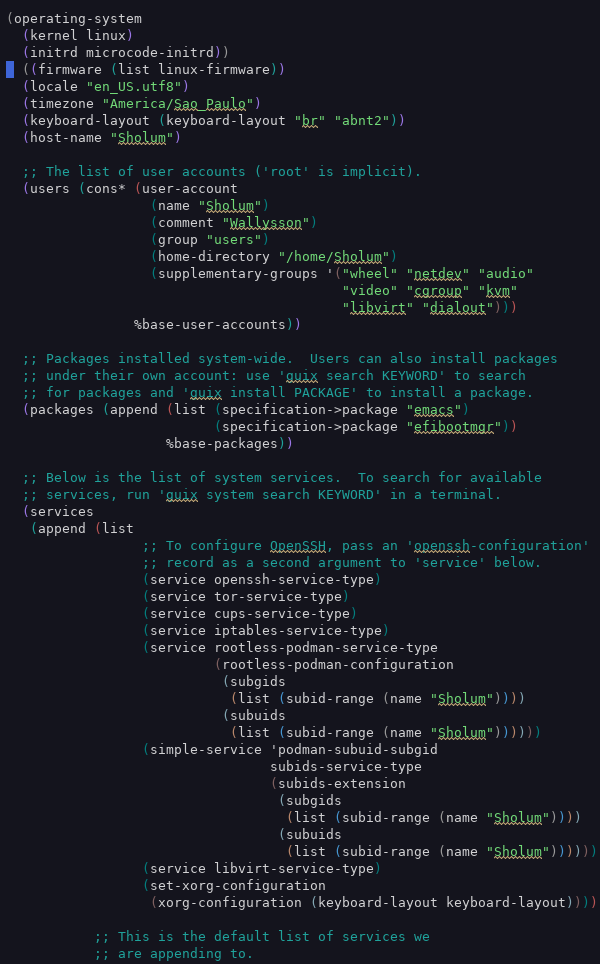
\includegraphics[height=1.2\textwidth]{~/Unicamp/MC504/Apresentação Guix/Configuração 1.png}
\end{minipage}%
\hfill
\begin{minipage}[c]{0.5\textwidth}
  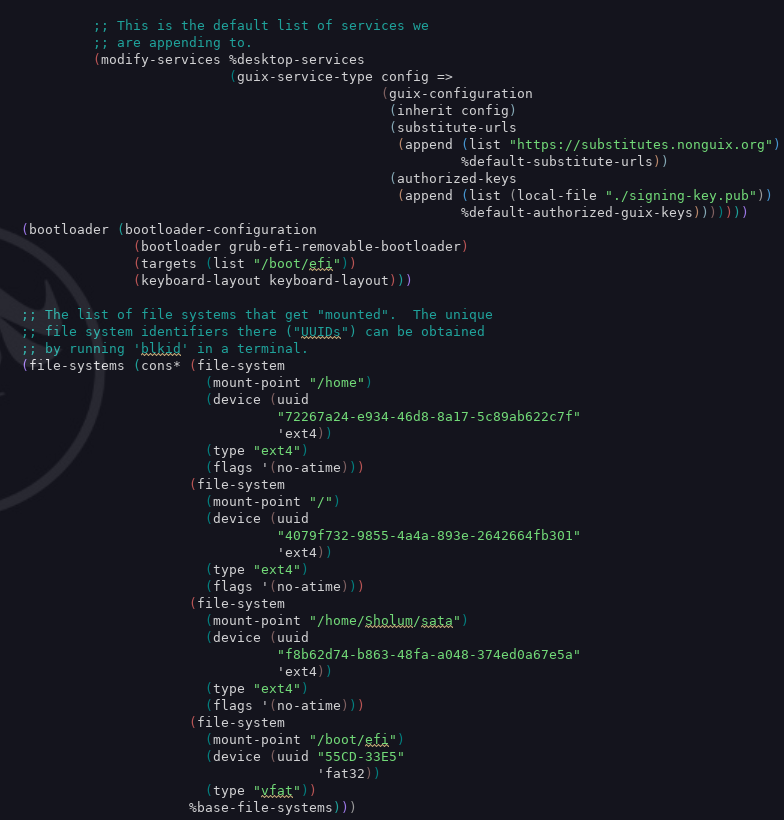
\includegraphics[height=1.2\textwidth]{~/Unicamp/MC504/Apresentação Guix/Configuração 2.png}
\end{minipage}
\end{frame}
\begin{frame}[label={sec:org6bf7dee}]{Por que Guile?}
Guile é uma implementação da linguagem Scheme, que por sua vez é um LISP, também parte do projeto GNU.

Por ser um Scheme é extremamente fácil de ser estendida através de macros e funções que rodam em tempo de
compilação, expansão, leitura ou execução.

Facilitando a criação de linguagens de domínio específicos (DSLs), como a própria configuração do Guix mostrada
acima.

Além disso, possui um rico ecossistema e uma comunidade fortemente ativa. Dentre projetos que utilizam Guile,
merecem destaque:
\end{frame}
\begin{frame}[label={sec:org949a59c}]{⁤}
\begin{enumerate}
\item Guix, que possui código Guile em seu core, além de ser a linguagem oficial de configuração;
\item \href{https://spritely.institute/goblins/}{Goblins}, projeto que traz uma série de abstrações para lidar com concorrência paralelismo em sistemas
distribuídos. Assim o programador pode se concentrar na programação de objetos e não na
arquitetura de protocolos;
\item \href{https://github.com/wingo/fibers}{Fibers}, projeto que traz um modelo de concorrência similar a implementada na linguagem Go para o Guile.
\end{enumerate}
\end{frame}
\begin{frame}[label={sec:orgfe6055a}]{Outras linguagens dentro do Guile}
O compilador do Guile também possui a implementação de outras linguagens, como EmacsLisp e ECMASscript.

Elas são compiladas para a mesma linguagem intermediária, chamada de tree-il, e por fim, executadas pela
mesma VM, permitindo assim a comunicação de diferentes linguagens entre si.

A comunidade vem buscando implementar uma versão de Python e Lua, mas toda linguagem é bem aceita!
\end{frame}
\begin{frame}[label={sec:orga9c5198}]{Aplicações práticas:}
Atualmente o uso de Guix vem crescendo muito na Indústria e na Academia, pelo mesmo motivo: reprodutibilidade

Como explicado anteriormente, é muito simples recriar e distribuir o sistema Guix com configurações e pacotes
específicos, facilitando a replicabilidade d pesquisas como mostram os papers
\href{https://www.biorxiv.org/content/10.1101/298653v2}{Reproducible genomics analysis pipelines with GNU Guix} e
\href{https://inria.hal.science/hal-01161771/en}{Reproducible and User-Controlled Software Environments in HPC with Guix}.
\end{frame}
\begin{frame}[label={sec:org5a8f814},fragile]{⁤}
 Outra experiência tem sido a minha no meu atual emprego na empresa \href{https://www.buzzlabs.com.br/}{Buzzlabs}, o uso do Guix tem sido estudado
para o desenvolvimento de contêineres e a realização de Deploy dos produtos da empresa.

A ideia é a criação de contêineres específicos para produtos específicos, utilizados tanto em desenvolvimento,
como na criação de testes, como na distribuição.

Guix possui uma série de ferramentas que podem ser utilizadas para facilitar esse processo, dentre eles, o
comando:
\begin{verbatim}
guix deploy [PATH]
\end{verbatim}
Que permite reconfigurar servidores não localmente.
\end{frame}
\begin{frame}[label={sec:org5d511c5}]{⁤}
Imagine o cenário em que nós possuímos temos que atualizar uma aplicação e, por conta disso, todos os nossos
servidores serão também atualizados.

O guix deploy facilita esse processo como mágica, carregando a mesma configuração em diferentes máquinas
através da web.

A lista de máquinas a serem reconfiguradas se encontram no arquivo, escrito em Guile, no PATH, como no exemplo
abaixo:
\end{frame}
\begin{frame}[label={sec:org851d22b}]{⁤}
\begin{center}
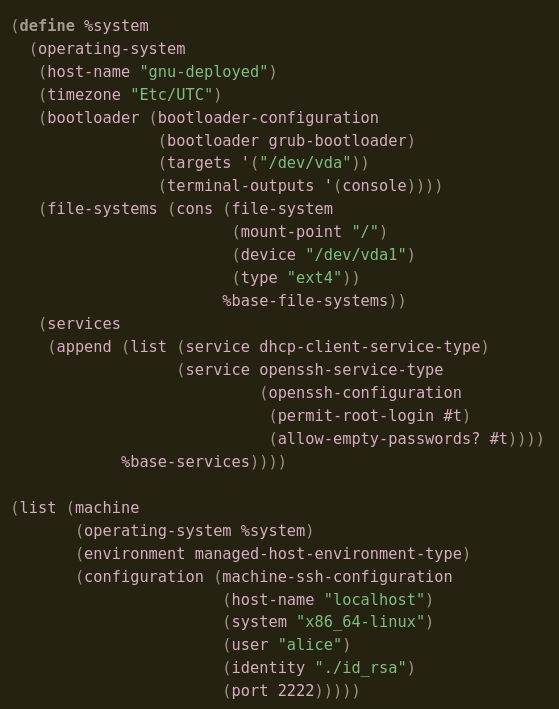
\includegraphics[height=220]{/home/Sholum/Unicamp/MC504/Apresentação Guix/Deploy.png}
\end{center}
\end{frame}
\begin{frame}[label={sec:orgb1c4a83}]{⁤}
\begin{center}

\includegraphics[height=220]{/home/Sholum/Unicamp/MC504/Apresentação Guix/Guix Logo.pdf}
\end{center}
\end{frame}
\end{document}
